
\section{Implementation}
\label{Implementation}

In diesem Kapitel wird die Implementation der einzelnen Container beschrieben, wie sie im Kapitel \ref{Architektur:Container} definiert wurden.

\subsection{ÖV-Güteklassen 2018 Generator}
\label{Implementation:ÖV-Güteklassen 2018 Generator}

\subsubsection{Datenaufbereitung}
\label{ÖV-Güteklassen 2018 Generator:Datenaufbereitung}

Der \acs{ÖV}-Güteklassen 2018 Generator operiert auf unterschiedlichen Daten von externen Datenquellen.
Diese Daten kommen in den verschiedensten Formaten daher und müssen für eine weitere Verarbeitung gefiltert, aufbereitet und optimiert werden.
Für eine einfache Handhabung wurde ein Docker-Setup gewählt.
Die Bedienung dieses Setups ist im Kapitel \ref{Softwaredokumentation} ausführlich beschrieben.

Grundsätzlich kann man sagen, dass zwei Docker-Container existieren, namentlich \emph{tooling} und \emph{db}.
Der Docker-Container \emph{tooling} nimmt Daten in gängigen Formaten entgegen oder bezieht diese von externen Diensten und bereitet sie so vor, dass diese vom Docker-Container \emph{db} in die Datenbank \emph{oevgk18} für eine Weitereverwendung des \acs{ÖV}-Güteklassen 2018 Generator geladen werden können.
Der Docker-Container \emph{db} sorgt ebenfalls dafür, dass beim Starten die nötigen Schemas, Stored Procedures und Indizes erstellt werden.

Im weiteren sind die Services, welche die beiden Docker-Container bereitstellen, anhand eines Datenflussdiagrams aufgeschlüsselt.
Für jeden Service im Docker-Container \emph{tooling} existiert ein Pendant im Docker-Container \emph{db}, welche die vorverarbeiteten Daten des Docker-Container \emph{tooling} entgegennimmt und in die Datenbank spielt.

\paragraph{OSM-Daten}~\\
\acs{OSM}-Daten werden von der Routing-Enginge für das Berechnen von Isolinien und für das Identifizieren von \acs{ÖV}-Haltestellen verwendet.
In Abbildung \ref{fig:dataflow-docker-setup-osm-data} ist ersichtlich, wie der Docker-Container \emph{tooling} die \acs{PBF}-Datei der Schweiz von einem externen Dienst~\cite{planet_osm_ch} bezieht und für die zwei vorhin erwähnten Zwecke verarbeitet.

\begin{figure}[ht]
    \centering
    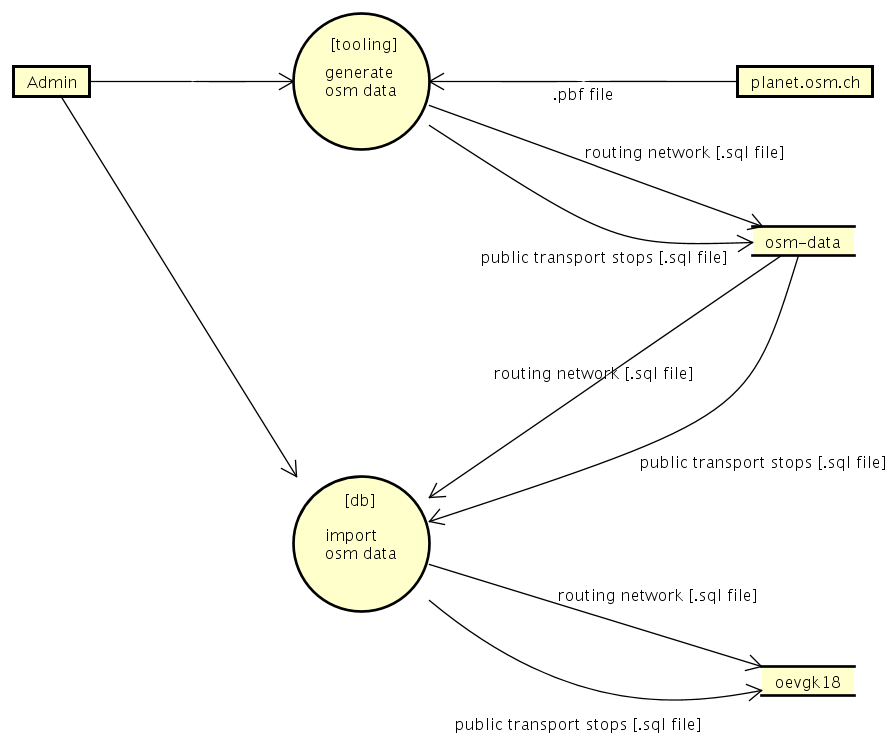
\includegraphics[width=0.8\linewidth]{projectdoc/img/dataflow-docker-setup-osm-data.png}
    \caption[Datenfluss Setup OSM-Daten]{Datenfluss Setup OSM-Daten}
    \label{fig:dataflow-docker-setup-osm-data}
\end{figure}

Das Routing-Netzwerk wird mithilfe des Tools \emph{OSM2PO}~\cite{OSM2PO} für pgrouting aufbereitet und als SQL-Datei bereitgestellt.
Die \acs{ÖV}-Haltestellen werden durch Osmosis~\cite{osmosis} gefiltert und ebenfalls in eine SQL-Datei exportiert.
Beide Tools werden durch separate Konfigurationen für unsere Zwecke konfiguriert.
So werden aus den \acs{OSM}-Daten für das Identifizieren von \acs{ÖV}-Haltestellen nur Nodes extrahiert, welche eine \emph{uic\_ref} besitzen. \ac{UIC}-Referenzen werden für die Identifizierung von \acs{ÖV}-Haltestellen verwendet.

\paragraph{GTFS-Daten}~\\
Die Fahrplandaten werden im Docker-Container \emph{tooling} von GTFS~\cite{gtfs_spec} heruntergeladen und im CSV-Format als TXT-Dateien bereitgestellt.
Diese wiederum können in einem nächsten Schritt durch den Docker-Container \emph{db} in die Datenbank gespielt werden.
Der Datenfluss ist in Abbildung \ref{fig:dataflow-docker-setup-gtfs-data} ersichtlich.

\begin{figure}[ht]
    \centering
    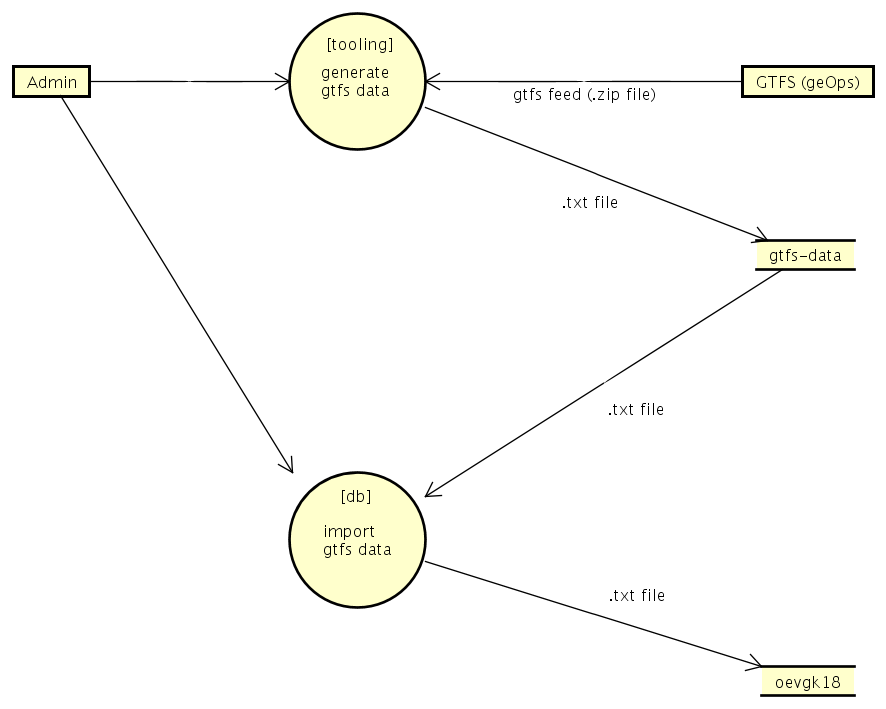
\includegraphics[width=0.8\linewidth]{projectdoc/img/dataflow-docker-setup-gtfs-data.png}
    \caption[Datenfluss Setup GTFS-Daten]{Datenfluss Setup GTFS-Daten}
    \label{fig:dataflow-docker-setup-gtfs-data}
\end{figure}

\paragraph{Terrain-Daten}~\\
Das Terrainmodell kann aufgrund der Grösse der Datei und aus lizenztechnischen Gründen nicht von einem externen Dienst bezogen und muss somit dem Service manuell als TIF-Datei bereitgestellt werden.
Diese Datei wird mit raster2pgsql~\cite{raster2pgsql}, einem Tool von PostGIS, welches Raster-Formate in ein Format konvertiert, welche in eine PostGIS-Tabelle geladen werden kann, verarbeitet.
Dieser Import wird dann vom Docker-Container \emph{db} durchgeführt.
Der Datenfluss ist in Abbildung \ref{fig:dataflow-docker-setup-terrain-data} ersichtlich.

\begin{figure}[ht]
    \centering
    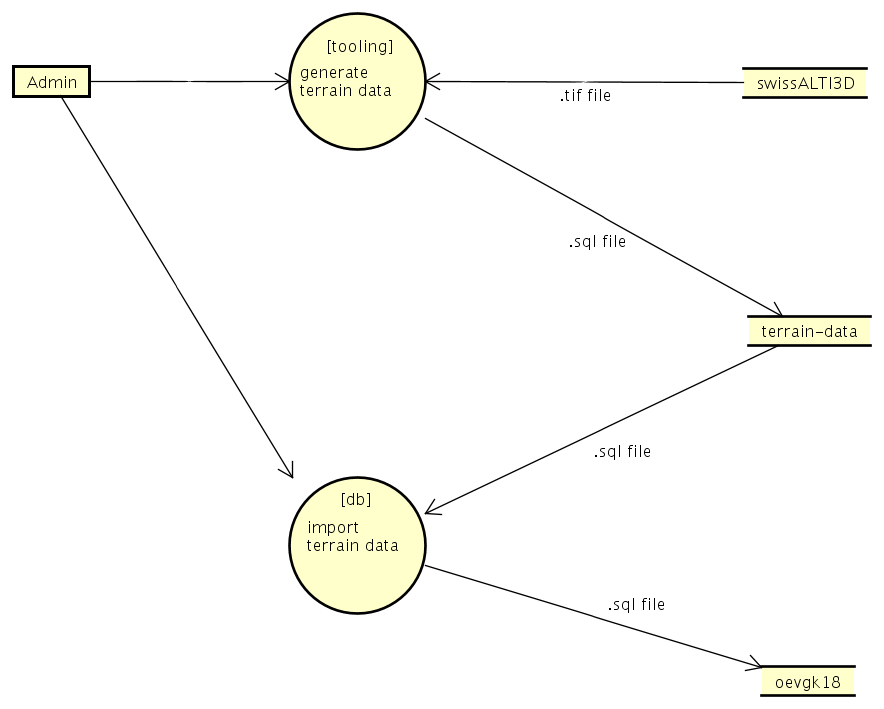
\includegraphics[width=0.8\linewidth]{projectdoc/img/dataflow-docker-setup-terrain-data.png}
    \caption[Datenfluss Setup Terrain-Daten]{Datenfluss Setup Terrain-Daten}
    \label{fig:dataflow-docker-setup-terrain-data}
\end{figure}

\subsubsection{Umsetzung Spezifikation}
\label{ÖV-Güteklassen 2018 Generator:Umsetzung Spezifikation}

\paragraph{Datenfluss}~\\
Durch die unterschiedliche Natur der Datenquellen und der Menge dieser ist es hilfreich, zu visualisieren, zu welchem Zeitpunkt, welche Daten zu welchen Zweck benötigt werden.
Wie in Abbildung \ref{fig:Flow_OeVGK_Brechnung} ersichtlich ist, werden die \acs{ÖV}-Güteklassen in fünf Schritten berechnet. 
In Abbildung \ref{fig:dataflow_OeV-Gueteklassen_2018_Generator} ist nun schematisch die Raison d’Être der Datenquellen ersichtlich.

\begin{figure}[ht]
    \centering
    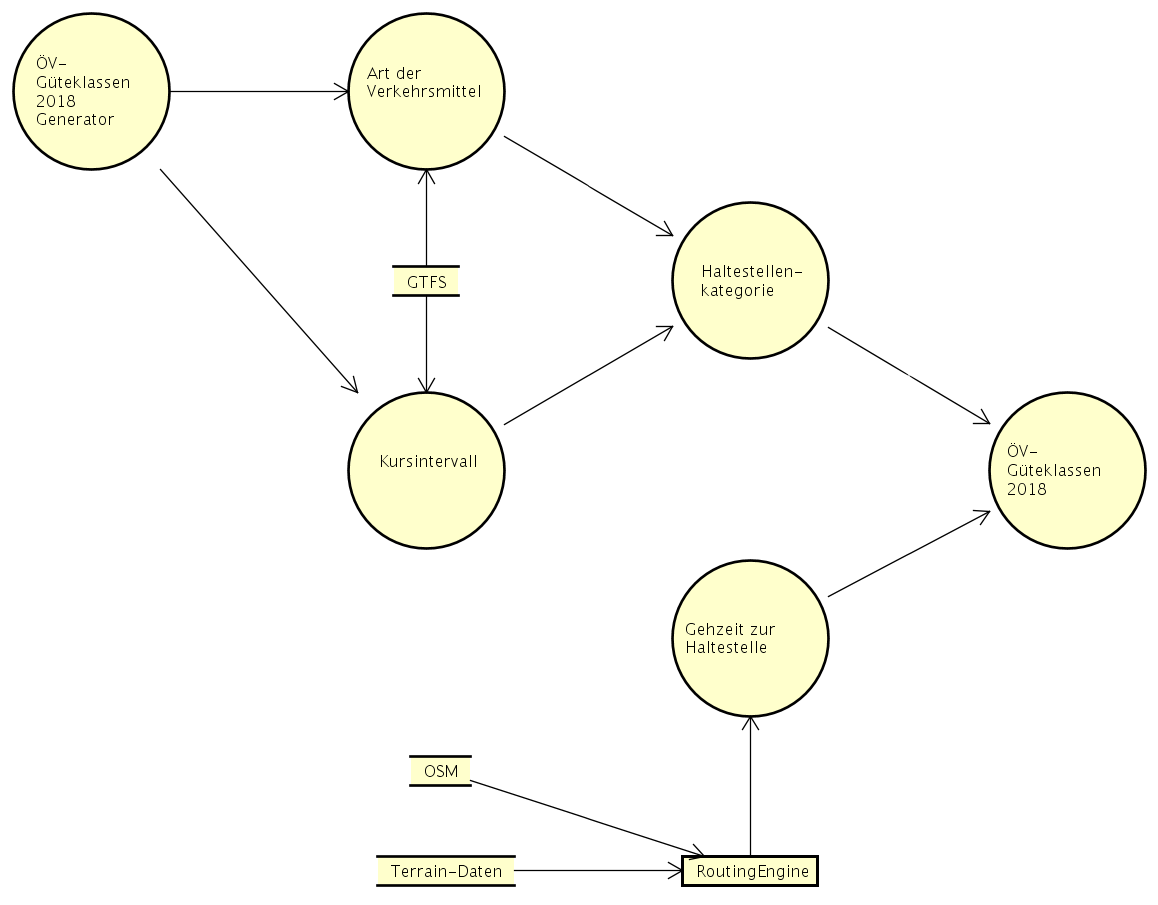
\includegraphics[width=1.0\linewidth]{projectdoc/img/dataflow_OeV-Gueteklassen_2018_Generator.png}
    \caption[Datenfluss ÖV-Güteklassen 2018 Generator]{Datenfluss ÖV-Güteklassen 2018 Generator}
    \label{fig:dataflow_OeV-Gueteklassen_2018_Generator}
\end{figure}

Die Datenquellen \emph{GTFS}, \emph{OSM} und \emph{Terrain-Daten} entsprechen an sich keinen separaten Datenquellen, sondern werden nur zum besseren Verständnis getrennt dargestellt.
Wie wir in Kapitel \ref{ÖV-Güteklassen 2018 Generator:Datenaufbereitung} gesehen haben, werden diese aufbereitet und optimiert in einer Datenbank \emph{oevgk18} gehalten.

\paragraph{Berechnung des Kursintervalls}~\\

Für die Berechnung des Kursintervalls wurde die Formel, wie sie in der Spezifikation (siehe Kapitel \ref{Berechnungsmethodik OeVGK18:Kursintervall}) definiert wurde, direkt umgesetzt.
Um alle Abfahrtszeiten einer Haltestelle zu erhalten, wurde zuerst eine SQL-Query für die GTFS-Datenbank formuliert, in der nach der \acs{UIC}-Referenz gefiltert wird.
Die Ausführung dieser Query dauerte allerdings ca. 1.7 Sekunden pro Haltestelle, was bei einer Gesamtzahl von 28'000 Haltestellen etwa 11 Stunden dauern würde.

Viel effizienter ist es, die Abfahrtszeiten für alle Haltestellen in einer einzelnen Abfrage zu aggregieren.
Diese ist in Listing \ref{listing:sql_query_departure_times} abgebildet.
Die optimierte SQL-Query dauert ca. 7 Sekunden für alle 28'000 Haltestellen, was eine drastische Verbesserung darstellt.

\begin{listing}[ht]
    \inputminted{sql}{projectdoc/listing/departure_time_cte.sql}
    \caption{Effiziente SQL-Query zur Abfrage aller Abfahrtszeiten an einem bestimmten Tag}
    \label{listing:sql_query_departure_times}
\end{listing}

\subsubsection{Mapping Verkehrsmittelgruppe und GTFS Route Type}
\label{ÖV-Güteklassen 2018 Generator:Mapping Verkehrsmittelgruppe und GTFS Route Type}

Die öffentlichen Verkehrsmittel werden in drei Verkehrsmittelgruppen gruppiert (siehe Kapitel \ref{Berechnungsmethodik OeVGK18:Art der Verkehrsmittel}).
Wie in Kapitel \ref{subsystem:GTFS} beschrieben, werden die Fahrplandaten im \acs{GTFS}-Format~\cite{gtfs_spec} gehalten. 
Es werden dabei 8 Verkehrsmittel-Typen definiert.
In Tabelle \ref{table:Mapping GTFS Route Type Verkehrsmittelgruppe} ist ein Mapping der definierten GTFS Route Typen und der Verkehrsmittelgruppen ersichtlich.

\begin{table}[ht]
    \centering
    \begin{tabular}[ht]{l l}
        \toprule
        \textbf{GTFS Route Type} 
                                & \textbf{Verkehrsmittelgruppe}\\
        \midrule
        0 (Tram, Streetcar, Light rail)
                                & C\\
        1 (Subway, Metro)
                                & -\\
        2 (Rail)
                                & A/B\\
        3 (Bus)
                                & C\\
        4 (Ferry)
                                & C\\
        5 (Cable car)
                                & -\\
        6 (Gondola, Suspended cable car)
                                & C\\
        7 (Funicular)
                                & C\\            
        \bottomrule
    \end{tabular}
    \caption{Mapping GTFS Route Type Verkehrsmittelgruppe}
    \label{table:Mapping GTFS Route Type Verkehrsmittelgruppe}
\end{table}
